%
% Niniejszy plik stanowi przykład formatowania pracy magisterskiej na
% Wydziale MIM UW.  Szkielet użytych poleceń można wykorzystywać do
% woli, np. formatujac wlasna prace.
%
% Zawartosc merytoryczna stanowi oryginalnosiagniecie
% naukowosciowe Marcina Wolinskiego.  Wszelkie prawa zastrzeżone.
%
% Copyright (c) 2001 by Marcin Woliński <M.Wolinski@gust.org.pl>
% Poprawki spowodowane zmianami przepisów - Marcin Szczuka, 1.10.2004
% Poprawki spowodowane zmianami przepisow i ujednolicenie 
% - Seweryn Karłowicz, 05.05.2006
% Dodanie wielu autorów i tłumaczenia na angielski - Kuba Pochrybniak, 29.11.2016

% dodaj opcję [licencjacka] dla pracy licencjackiej
% dodaj opcję [en] dla wersji angielskiej (mogą być obie: [licencjacka,en])
\documentclass[licencjacka]{pracamgr}


% Dane magistranta:
\autor{Imię Nazwisko}{123456}


% Dane magistrantów:
%\autor{Autor Zerowy}{342007}
%\autori{Autor Pierwszy}{342013}
%\autorii{Drugi Autor-Z-Rzędu}{231023}
%\autoriii{Trzeci z Autorów}{777321}
%\autoriv{Autor nr Cztery}{432145}
%\autorv{Autor nr Pięć}{342011}

\title{Interaktywna eksploracja i dopasowanie lokalnie optymalnych struktur biopolimerów z wykorzystaniem metod wirtualnej rzeczywistości}


%\tytulang{An implementation of a difference blabalizer based on the theory of $\sigma$ -- $\rho$ phetors}

%kierunek: 
% - matematyka, informacyka, ...
% - Mathematics, Computer Science, ...
\kierunek{bioinformatyka}

% informatyka - nie okreslamy zakresu (opcja zakomentowana)
% matematyka - zakres moze pozostac nieokreslony,
% a jesli ma byc okreslony dla pracy mgr,
% to przyjmuje jedna z wartosci:
% {metod matematycznych w finansach}
% {metod matematycznych w ubezpieczeniach}
% {matematyki stosowanej}
% {nauczania matematyki}
% Dla pracy licencjackiej mamy natomiast
% mozliwosc wpisania takiej wartosci zakresu:
% {Jednoczesnych Studiow Ekonomiczno--Matematycznych}

% \zakres{Tu wpisac, jesli trzeba, jedna z opcji podanych wyzej}

% Praca wykonana pod kierunkiem:
% (podać tytuł/stopień imię i nazwisko opiekuna
% Instytut
% ew. Wydział ew. Uczelnia (jeżeli nie MIM UW))
\opiekun{dr. hab. Filigrana Fifaka\\
  Instytut Blabalii Fetorycznej\\
  }

% miesiąc i~rok:
\date{Maj 2017}

%Podać dziedzinę wg klasyfikacji Socrates-Erasmus:
\dziedzina{ 
%11.0 Matematyka, Informatyka:\\ 
%11.1 Matematyka\\ 
11.2 Statystyka\\ 
%11.3 Informatyka\\ 
%11.4 Sztuczna inteligencja\\ 
%11.5 Nauki aktuarialne\\
%11.9 Inne nauki matematyczne i informatyczne
}

%Klasyfikacja tematyczna wedlug AMS (matematyka) lub ACM (informatyka)
\klasyfikacja{D. Software\\
  D.127. Blabalgorithms\\
  D.127.6. Numerical blabalysis}

% Słowa kluczowe:
\keywords{bioinformatyka, wirtualna rzeczywistość, podobieństwo strukturalne, RNA, DNA, białka, biopolimery, uliniowienie }

% Tu jest dobre miejsce na Twoje własne makra i~środowiska:
\newtheorem{defi}{Definicja}[section]

\usepackage{graphicx}
\usepackage[export]{adjustbox}
\usepackage{float}
\usepackage{amsmath}
% koniec definicji

\begin{document}

\maketitle

%tu idzie streszczenie na strone poczatkowa
\begin{abstract}
W pracy przedstawiono implementację programu narzędziowego służącego do interaktywnej eksploracji cząsteczek biopolimerów (polinukleotydów i polipeptydów) w poszukiwaniu miejsc optymalnych ze względu na lokalne podobieństwo strukturalne. W pracy szeroko zastosowano metody wirtualnej rzeczywistości wraz z obsługą urządzenia haptycznego Sensable Phantom Omni.
\end{abstract}

\tableofcontents
%\listoffigures
%\listoftables

\chapter*{Wprowadzenie}
\addcontentsline{toc}{chapter}{Wprowadzenie}
Biopolimery, a w szczególności kwasy nukleinowe i polipeptydy stanowią fundamenty życia. W każdej komórce oraz w całym organizmie są one odpowiedzialne za najważniejsze funkcje związane z odżywianiem, rozmnażaniem czy obroną przed patogenami. Dzięki kwasom nukleinowym możliwe jest przenoszenie informacji genetycznej, biorą one udział w syntezie białek, a także mają funkcję enzymatyczne. Polipeptydy i białka zaś są składnikami budulcowymi wielu organów, pełnią funkcje hormonalne czy regulatorowe.

Pomimo odmiennych składników budulcowych – nukleotydów i aminokwasów – w obu przypadkach wymienionych biopolimerów ich funkcja wynika bezpośrednio ze struktury przestrzennej, która to za hipotezą Anfinsena [1] jest ściśle zdeterminowana przez sekwencję nukleotydów czy aminokwasów.

Struktura przestrzenna biopolimerów stanowi obecnie przedmiot niezwykle intensywnych badań na całym świecie. Jest to bardzo ważne zagadnienie integrujące ze sobą grupy naukowców z dziedzin, które jeszcze na przełomie wieków miały ze sobą niewiele wspólnego. Do grona biologów i chemików dołączyli matematycy, fizycy oraz informatycy wspólnie tworząc bardzo nowatorskie narzędzia ułatwiające modelowanie i tworzenie symulacji zachodzących w skali molekularnej. W badania nad strukturami przestrzennymi biopolimerów zaangażowane są największe na świecie ośrodki naukowe, korporacje farmaceutyczne czy agencje rządowe. Badanie interakcji receptorów z ligandami, projektowanie nowych leków czy terapie celowane to tylko wąski wycinek zagadnień związanych z tymi pracami.

Intensywny rozwój narzędzi bioinformatycznych znacznie ułatwił i przyspieszył te badania. Obecnie najwydajniejsze komputery bez przerwy prowadzą obliczenia optymalnie pofałdowanych białek, kwasów nukleinowych czy prowadzą symulacje dynamiki molekularnej. Jest to dziedzina w której niemalże każdego roku dokonuje się przełomowych odkryć i prawdopodobnie jeszcze przez długi czas to się nie zmieni. Wystarczy przytoczyć wyniki odbywającego się co dwa lata międzynarodowego konkursu CASP na najlepsze przewidywanie struktury białka, który za każdym razem przynosi coraz to doskonalsze wyniki. 

Nie mniej ważnym od samych badań jest prezentacja ich wyników szerokiemu gronu odbiorców. Same efektowne wizualizacje wyników badań nie zawsze są wystarczające, coraz częściej chcemy wchodzić w bezpośrednią interakcję ze światem do którego dostępu nie mieliśmy nigdy wcześniej za pośrednictwem naszych zmysłów. W ostatnim czasie coraz częściej sięga się także do rozwiązań z zakresu wirtualnej rzeczywistości. 

Mianem wirtualnej rzeczywistości (ang. virtual reality) określamy sztuczne, wykreowane przy pomocy technologii informatycznych multimedialne projekcje przestrzeni, przedmiotów czy zdarzeń. Na obecnym poziomie rozwoju technologii wirtualna rzeczywistość umożliwia człowiekowi wchodzenie w interakcję z tym środowiskiem przede wszystkim za pośrednictwem zmysłów wzorku, słuchu czy dotyku. 

Wirtualna rzeczywistość w dzisiejszym świecie zyskuje coraz to większą popularność w wielu dziedzinach życia, od zastosowań czysto rozrywkowych po zaawansowane projekty naukowe, przemysłowe czy wojskowe. Postępująca od wielu lat miniaturyzacja, rozwój nowych algorytmów czy drastyczne zwiększenie wydajności obliczeniowej sprzętu komputerowego jedynie przyspiesza ten proces. 
\\
\\
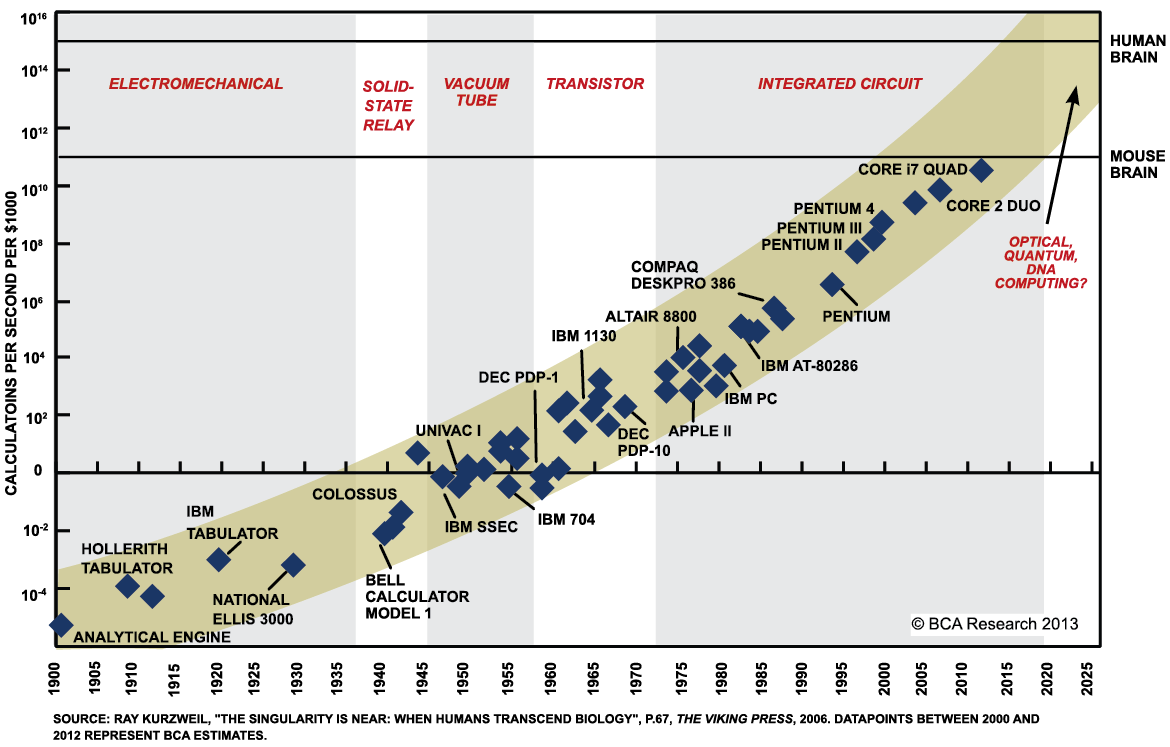
\includegraphics[scale=0.35,center]{MooresLaw}
\\
\\
Elementami niezbędnymi do prawidłowego wykreowania wirtualnego środowiska jest zarówno dedykowane oprogramowanie jak i sprzęt konieczny do przekazywania informacji zwrotnych do użytkownika. Rzeczywistość wirtualna aby zostać możliwie najlepiej zinterpretowana przez ludzki mózg musi jak najbardziej przypominać rzeczywistość w której żyjemy na co dzień. Aby sprostać temu zadaniu najczęściej reprezentuje się ją w postaci trójwymiarowych scen. Tylko ten jeden czynnik powoduje, że do poprawnej symulacji niezbędne są nowoczesne, wysokowydajne procesory i karty graficzne będące w stanie przeprowadzić niezbędne obliczenia.

Jak już wspomniano wirtualna rzeczywistość może znajdować zastosowanie także w nauce w szczególności w dziedzinach w których obiekty zainteresowań są zbyt małe aby być widoczne gołym okiem, takie jak cząsteczki chemiczne lub pojedyncze atomy. Istnieje cały szereg programów przeprowadzających np. symulacje oddziaływań międzycząsteczkowych, zwijania białek (ang. protein folding) czy przeprowadzających obliczenia dynamiki molekularnej (ang. molecular dynamics), a także umożliwiających wizualizację tych symulacji. Stosunkowo niewiele jednak jest rozwiązań dedykowanych wirtualnej rzeczywistości, które mogłyby umożliwić interakcję ze sprzężeniem zwrotnym. 
	
Pracownie Laboratorium Biofizyki na Wydziale Fizyki Uniwersytetu Warszawskiego dysponują sprzętem niezbędnym do realizacji takich zadań. Urządzenie haptyczne Sensable Phantom Omni jest przykładem trójwymiarowego wskaźnika ze zwrotną projekcją momentów sił, którego wykorzystanie otwiera całe spektrum nowych możliwości związanych z realizacją projektów wirtualnej rzeczywiści w biofizyce molekularnej. 
	
Z punktu widzenia osoby zajmującej się szeroko pojętą biofizyką molekularną na szczególną uwagę zasługują związki

\chapter*{Cel i zakres pracy}
\addcontentsline{toc}{chapter}{Cel i zakres pracy}

W ramach niniejszej pracy została przedstawiona implementacja narzędzia z pogranicza wirtualnej rzeczywistości i biofizyki molekularnej. Program służący do interaktywnej eksploracji struktur biopolimerów w poszukiwaniu regionów optymalnych ze względu na jakość dopasowania strukturalnego wzorca (ang. template) i fragmentów cząsteczki celu (ang. target). Jakość znalezionego dopasowania odwzorowuje zwrotna projekcja momentów sił do urządzenia haptycznego. 
	
Program pracuje w formie wtyczki do pakietu PyMOL, do swojego działania wykorzystuje urządzenia i metody wirtualnej rzeczywistości, bioinformatyczne algorytmy pomiaru jakości dopasowania struktur (RMSD), algorytmy wyszukujące optymalne dopasowanie (uliniowienie) struktur oraz algorytmy maksymalizujące stopień dopasowania struktur (algorytm Kabsch'a).

Poprawne uruchomienie i korzystanie z prezentowanego programu wymaga zestawienia stanowiska pracy składającego się z elementów przedstawionych na diagramie:
	
\textbf{TODO:} diagram prezentujący stanowisko pracy (komputer+haptic+vrpn+pymol)

W dalszej części pracy szczegółowo zostanie opisane stanowisko pracy.

\chapter{Podstawy teoretyczne}
W tym rozdziale zaprezentowano podstawowe twierdzenia i teorię leżącą u podstaw niniejszej pracy. Skupiono się głównie na zagadnieniach związanych z wykorzystanymi algorytmami oceny podobieństwa strukturalnego, przekształceniami geometrycznymi oraz metodami dopasowania lokalnego (uliniawiania) struktur chemicznych.

\section{RMSD}
Efektywna ocena podobieństwa struktur chemicznych jest jednym z kluczowych elementów niniejszej pracy. W bioinformatyce istnieje kilka sposobów oszacowania tej wartości: obok GDT (ang. global distance test) i TM-score (ang. template modeling score) najpopularniejsza i stosunkowo prosta w zastosowaniu jest miara odchylenia średniokwadratowego - RMSD (ang. root-mean-squared deviation). 

Ocena podobieństwa metodą RMSD polega na obliczeniu średniokwadratowej odległości pomiędzy współrzędnymi atomów zawartych w strukturze wzorca (ang. template) i w odpowiednim fragmencie cząsteczki celu (ang. target). W tym przypadku jednostką najczęściej jest \AA (angstrom). Dwie struktury są tym bardziej do siebie podobne im bliższa zeru jest wartość RMSD.

\boldmath{
$$
RMSD(p,q) = \sqrt{\frac{1}{N}\sum_{i=1}^{N}||p_i-q_i||^{2}} = 
$$
$$ 
= \sqrt{\frac{1}{N}\sum_{i=1}^{N}((p_{ix}-q_{ix})^{2}+(p_{iy}-q_{iy})^{2}+(p_{iz}-q_{iz})^{2})}
$$
}
gdzie:

\textbf{$p$} - wektor współrzędnych struktury wzorca

\textbf{$q$} - wektor współrzędnych wybranego regionu w strukturze celu

\textbf{$N$} - długość wektorów współrzędnych \textbf{$p$} i \textbf{$q$}
\\
\\
O ile same obliczenia są trywialne, to dobór danych wejściowych do algorytmu RMSD może stanowić poważne wyzwanie. 

W tym przypadku dane pochodzą z zewnętrznej aplikacji, która wykonuje procedurę dopasowania (uliniowienia) struktur wzorca i celu i odnajduje takie regiony, których miara podobieństwa nie przekracza zadanego progu (ang. threshold). Wynikiem takiej procedury są dane mapujące (ang. mapping file) zawierające informację o lokalizacji \textit{regionów podobnych} do struktury wzorca w cząsteczce celu. Takimi regionami mogą być dowolne struktury drugorzędowe (w szczególności alfa-helisy czy beta-harmonijki) lub trzeciorzędowe.

\begin{figure}[H]
\centering
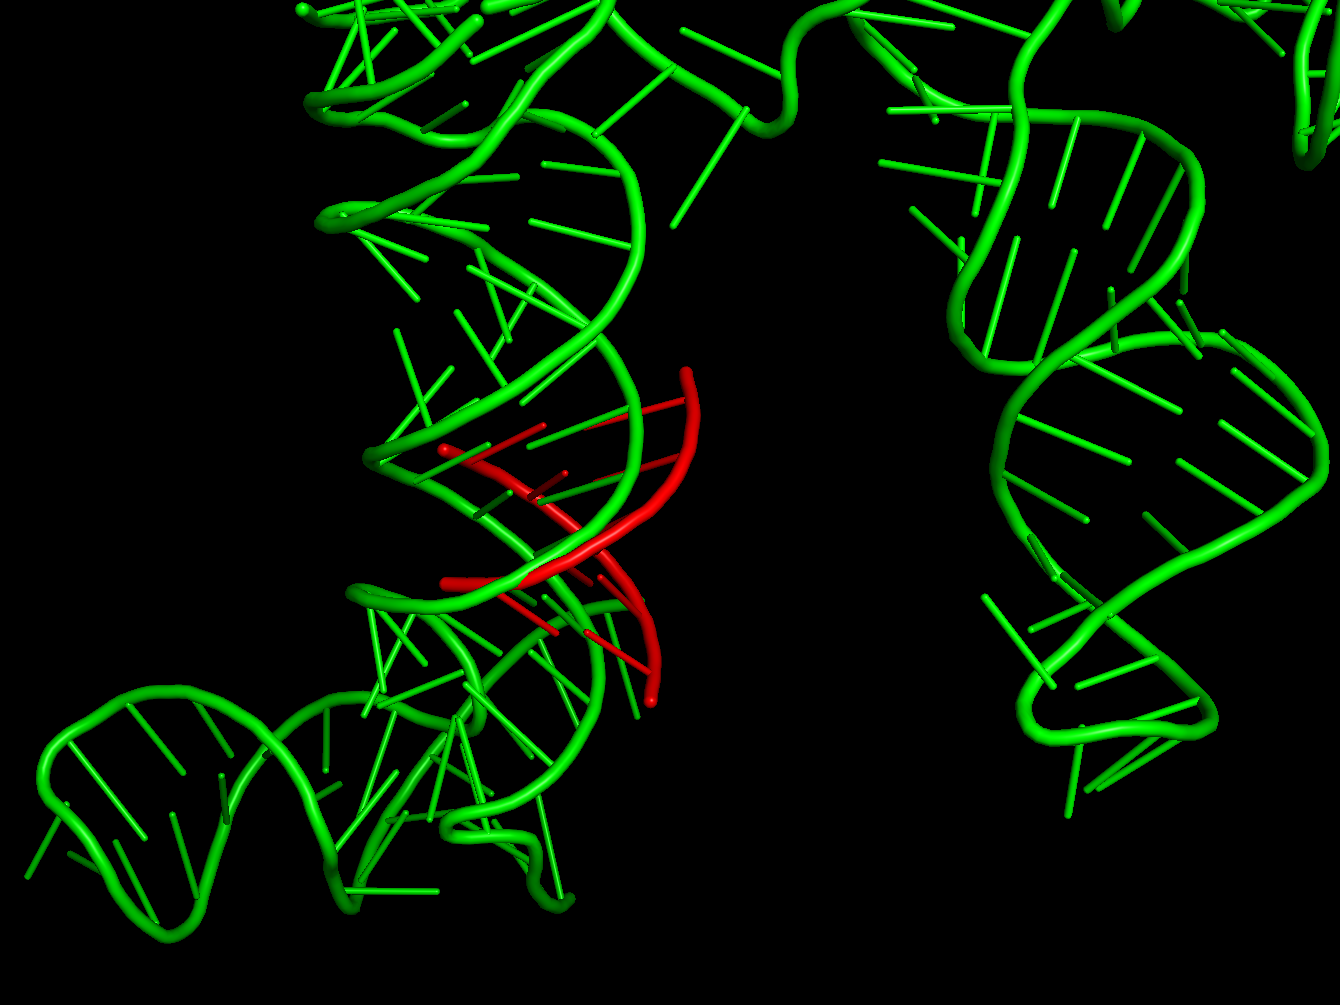
\includegraphics[scale=0.25]{rmsd3}
\caption{Przykładowe dopasowanie struktury wzorca (czerwona) do podobnego regionu struktury celu (zielona), RMSD=3.985}
\end{figure}

%
%\begin{figure}[H]
%\centering
%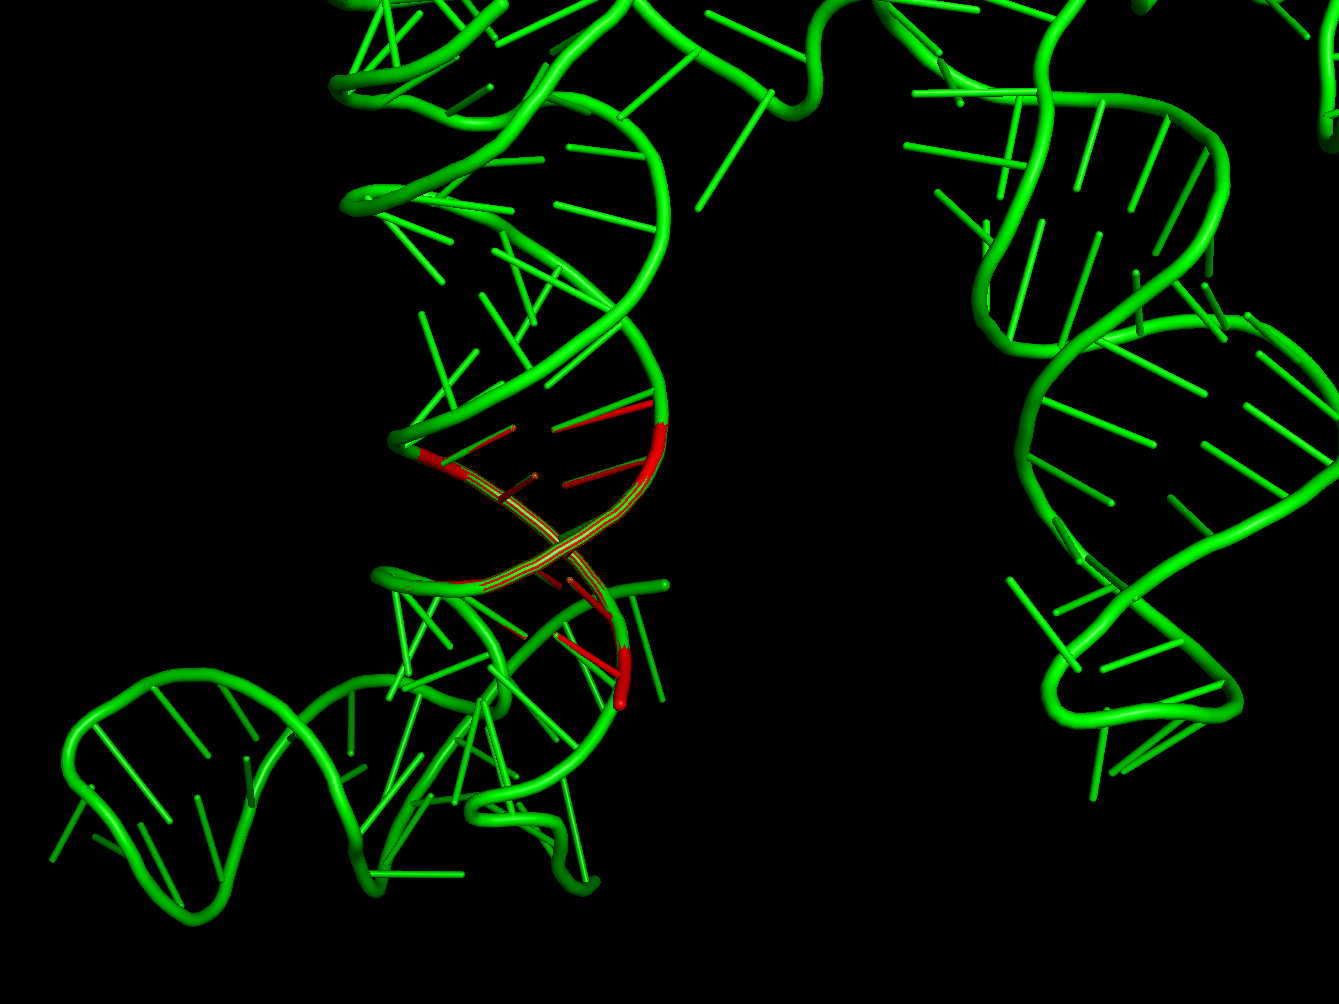
\includegraphics[scale=0.25]{rmsd0}
%\caption{Przykładowe dopasowanie struktury wzorca (czerwona) do %podobnego regionu struktury celu (zielona), RMSD=0}
%\end{figure}

\section{Algorytm Kabsch'a}
RMSD jest jedną podstawowych miar podobieństwa strukturalnego wykorzystywanych w bioinformatyce. Jednym ze znanych sposobów minimalizacji jego wartości jest optymalna translacja i rotacja struktury wzorca nad wybranym regionem struktury celu w taki sposób aby obie struktury zostały jak najlepiej na siebie nałożone. Sposób wyznaczania tych optymalnych transformacji opisał opisał w 1976 roku w swojej pracy [2] Wolfgang Kabsch.

Algorytm startuje z dwoma wektorami współrzędnych $p$ i $q$ o długości $N$. Wektor $p$ stanowi zbiór współrzędnych kartezjańskich struktury wzorca, $q$ - wybranego regionu struktury celu:
$$
p=
\begin{pmatrix}
 x_{p1} & y_{p1} & z_{p1} \\
 x_{p2} & y_{p2} & z_{p2} \\
 \vdots & \vdots & \vdots \\
 x_{pN} & y_{pN} & z_{pN}
\end{pmatrix}
$$
$$
q= 
\begin{pmatrix}
 x_{q1} & y_{q1} & z_{q1} \\
 x_{q2} & y_{q2} & z_{q2} \\
 \vdots & \vdots & \vdots \\
 x_{qN} & y_{qN} & z_{qN}
\end{pmatrix}
$$
\\
Algorytm Kabsch'a składa się z 3 kroków:
\begin{enumerate}
\item \textbf{Translacja} \\
W pierwszym kroku należy dokonać obliczenia punktów środkowych (centroidów) obu struktur ($Cp$ i $Cq$) i dokonać przesunięcia struktury wzorca o wektor $T$ rozpięty pomiędzy tymi punktami tak, aby centroidy nałożyły się na siebie. Jako punkt środkowy można wybrać środek masy lub środek geometryczny, np: 
$$Cp = (Cp_x, Cp_y, Cp_z)$$
gdzie:
$$Cp_x = \frac{1}{N}\sum_{i=1}^{N}{x_{pi}}$$
$$Cp_y = \frac{1}{N}\sum_{i=1}^{N}{y_{pi}}$$
$$Cp_z = \frac{1}{N}\sum_{i=1}^{N}{z_{pi}}$$
oraz
$$Cq = (Cq_x, Cq_y, Cq_z)$$
gdzie:
$$Cq_x = \frac{1}{N}\sum_{i=1}^{N}{x_{qi}}$$
$$Cq_y = \frac{1}{N}\sum_{i=1}^{N}{y_{qi}}$$
$$Cq_z = \frac{1}{N}\sum_{i=1}^{N}{z_{qi}}$$
zatem wektor translacji:
$$ T = |Cp-Cq| = $$
$$=(|Cp_x-Cq_x|,|Cp_y-Cq_y|,|Cp_z-Cq_z|)$$
\item \textbf{Macierz kowariancji} \\
Macierz kowariancji jest niezbędna do oceny tego jak bardzo obie struktury się od siebie różnią.
\item \textbf{Optymalna macierz rotacji}


\end{enumerate}



\section{Pole siłowe}
todo

\section{Przekształcenia geometryczne}
Przekształcenia geometryczne w przestrzeni trójwymiarowej stanowią elementarne operacje intensywnie używane w niniejszej pracy. Do podstawowych przekształceń zaliczamy skalowanie, translacje i rotacje. Wszystkie te operacje można praktycznie zrealizować na kilka sposobów. Optymalne metody numeryczne realizujące te przekształcenia są zatem priorytetem i muszą w minimalnym stopniu obciążać komputerowe jednostki obliczeniowe. Niezbędne jest także stosowanie konwersji pomiędzy różnymi formatami danych zawierających informacje o przekształceniach czy nawet samymi sposobami przekształcania występującymi w pakiecie PyMOL i VRPN. 

TODO: trochę ogólnych formalizmów matematycznych „czym są przekształcenia”

\subsection{Skalowanie}
	Skalowanie jest jednym z najprostszych przekształceń. Polega na przemnożeniu każdej składowej wektora współrzędnych obiektu określonego w przestrzeni trójwymiarowej przez dodatnio określony wektor skalujący C' lub wartość skalarną C zwanymi współczynnikami skalowania. Geometryczna intuicja stojąca za operacją skalowania polega na takim przekształceniu współrzędnych wyjściowego obiektu, że w zależności od wartości  współczynnika skalującego może zostać:
	
zmniejszony, gdy C<1

powiększony, gdy C>1

niezmieniony, gdy C=1

\subsection{Translacje}

\subsection{Rotacje}
W geometrii euklidesowej translacją nazywamy takie przekształcenie geometryczne, które przenosi każdy punkt określony w przestrzeni o dowolny wektor V. Dla przykładu punkt:
A=(Ax, Ay, Az)
przesunięty o wektor:
V=(Vx, Vy, Vz)
będzie miał współrzędne:
A\=(Ax+Vx, Ay+Vy, Az+Vz)

Translacje są powszechną operacją używaną między innymi w grafice komputerowej. Z tego faktu wynika, że tego typu

Skalowanie jest operacją polegającą na przemnożeniu wektora punktów określonego w przestrzeni o dowolną wartość skalarną będącą 

Przesunięcia o wektor czyli translacje stanowią pierwszy z tych elementów. Formalnie definicja translacji


\section{Metody lokalnego dopasowania struktur chemicznych}
todo: streszczenie doktoratu PD

Ważnym problemem jest przeszukiwanie struktury trójwymiarowej 

	
\chapter{Urządzenie haptyczne Sensable Phantom Omni}
Nadrzędnym celem wirtualnej rzeczywistości jest możliwie wierne odtworzenie rzeczywistości w świecie komputerowym oraz umożliwienie użytkownikowi wchodzenie w interakcję z tymi symulacjami. Między innymi do tego celu powstało urządzenie Phantom Omni opracowane przez firmę Sensable (obecnie Geomagic).
\\
\\
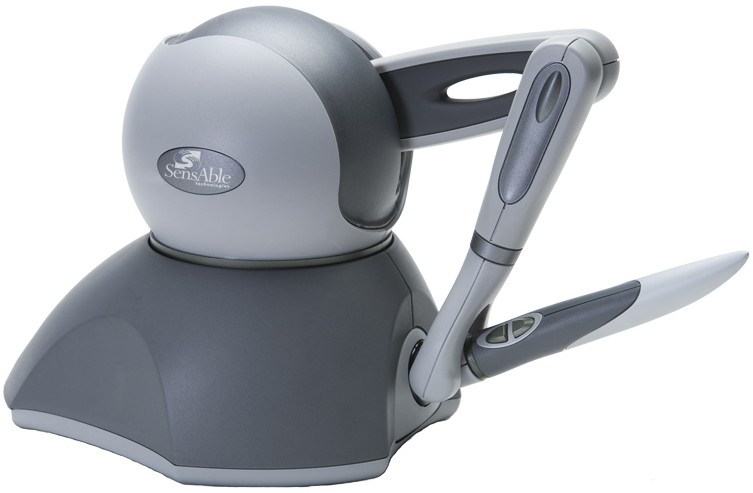
\includegraphics[scale=0.5,center]{Sensable_Phantom_Omni}
\\
\\
\section{Opis urządzenia}
Urządzenie haptyczne Sensable Phantom Omni jest trójwymiarowym wskaźnikiem o 6 stopniach swobody wskazywania pozycji i orientacji obiektu z możliwością programowego sterowania zwrotną projekcją momentów sił – o trzech stopniach swobody. 

Jest to urządzenie wykorzystywane w profesjonalnych rozwiązaniach z zakresu wirtualnej rzeczywistości czy modelowania trójwymiarowego. Producent wraz z urządzeniem dostarcza  sterowniki oraz pakiet bibliotek programistycznych OpenHaptics umożliwiających tworzenie dowolnego oprogramowania w pełni wykorzystującego możliwości urządzenia. 

Producent w nocie katalogowej podaje nominalną rozdzielczość zwracanej pozycji na około 450dpi (0.055mm) oraz tolerancję orientacji na około 5\% co w zupełności wystarcza do prezentowanych zastosowań.

\textbf{TODO:} szczegolowy opis + rysunki
	
\section{Wymagania sprzętowe}

	Urządzenia Sensable Phantom Omni w które wyposażona jest Pracownia Biofizyki Wydziału Fizyki Uniwersytetu Warszawskiego posiadają dwa rodzaje interfejsów: FireWire (IEEE-1394a) oraz Ethernet.
	
W pierwszym przypadku (na którym bazuje niniejsza praca) producent zaleca stosowanie kontrolerów IEEE-1394a opartych o chipset firmy NEC lub VIA. Ponadto w związku z zaprzestaniem wspierania tego standardu przez firmę Microsoft w systemach operacyjnych nowszych niż Windows 8?? wsparcie firmy Sensable dla tych urządzeń również zostało wstrzymane. Ta sytuacja rodzi cały szereg problemów już na etapie instalacji sterowników, w praktyce niemalże uniemożliwiając pracę z tym urządzeniem w nowszych systemach operacyjnych. 

Rozwiązaniem problemu może okazać się praca na starszych wersjach sterowników lub zastosowanie systemu GNU/Linux na którym wsparcie jest wciąż zapewnione.
	
\textbf{TODO:} dopisac tu cos jeszcze...

\section{Struktura oprogramowania OpenHaptics Toolkit}

OpenHaptics Toolkit jest bogatym pakietem oprogramowania dostarczanego przez firmę Sensable. Umożliwia on dostęp do niskopoziomowych funkcji urządzenia Phantom Omni tworząc przyjazną dla programisty abstrakcję. 
\\
\\
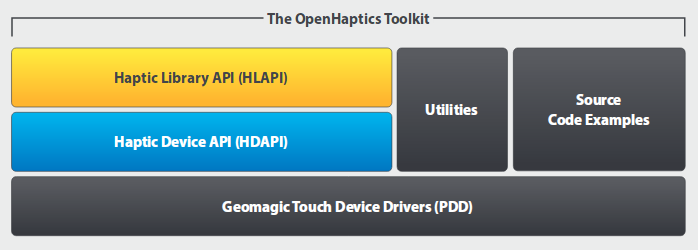
\includegraphics[scale=0.5,center]{openhaptics}
\\
\\
Na OpenHaptics Toolkit składa się kilka elementów składowych, są to:
sterowniki PDD (Phantom Device Drivers) – sterowniki wszystkich urządzeń haptycznych oferowanych przez producenta:

- Haptic Device API (HDAPI) – niskopoziomowe API umożliwiające bezpośredni dostęp do funkcji sterujących projekcją sił i pobieraniem danych o pozycji i orientacji wskaźnika

- Haptic Library API (HLAPI) – wysokopoziomowe API zaprojektowane głównie pod kątem zgodności składniowej z OpenGL API

\section{Przykłady wykorzystania}
tu beda jakies rzeczy...


\chapter{Biblioteka VRPN}
ll

\section{Opis pakietu}
opisik

\section{Dostosowanie VRPN do wymagań niniejszej pracy}
opis

\section{Kompilacja i uruchomienie}
kompilacja i uruchomienie

\chapter{Pakiet PyMOL}
opis pakietu

\section{Opis Oprogramowania}
opisik

\section{Sposób tworzenia wtyczek}
opisik

\chapter{Opis stanowiska laboratoryjnego}



\chapter{Podstawowe pojęcia}\label{r:pojecia}

Pojęciem pierwotnym blabalii fetorycznej jest \emph{blaba}.
Blabaliści nie podają jego definicji, mówiąc za Ciach-Pfe t-\=am
K\^un (fooistyczny mędrzec, XIX w. p.n.e.):
\begin{quote}
  Blaba, który jest blaba, nie jest prawdziwym blaba.

\raggedleft\slshape tłum. z~chińskiego Robert Blarbarucki
\end{quote}

\section{Definicje}

Oto dwie definicje wprowadzające podstawowe pojęcia blabalii
fetorycznej:

\begin{defi}\label{skupienie}
  Silny, zwarty i gotowy fetor bazowy nazwiemy \emph{skupieniem}.
\end{defi}

\begin{defi}\label{fetor}
  \emph{Fetorem} nazwiemy skupienie blaba spełniające następujący
  \emph{aksjomat reperkusatywności}:
  $$\forall \mathcal{X}\in Z(t)\ \exists
  \pi\subseteq\oint_{\Omega^2}\kappa\leftrightarrow 42$$
\end{defi}


\section{Blabalizator różnicowy}

Teoretycy blabalii (zob. np. pracę~\cite{grglo}) zadowalają się
niekonstruktywnym opisem natury fetorów.

Podstawowym narzędziem blabalii empirycznej jest blabalizator
różnicowy.  Przyrząd ten pozwala w~sposób przybliżony uzyskać
współczynniki rozkładu Głombaskiego dla fetorów bazowych
i~harmonicznych.  Praktyczne znaczenie tego procesu jest oczywiste:
korzystając z~reperkusatywności pozwala on przejść do przestrzeni
$\Lambda^{\nabla}$, a~tym samym znaleźć retroizotonalne współczynniki
semi-quasi-celibatu dla klatek Rozkoszy (zob.~\cite{JR}).

Klasyczne algorytmy dla blabalizatora różnicowego wykorzystują:
\begin{enumerate}
\item dualizm falowo-korpuskularny, a w szczególności
  \begin{enumerate}
  \item korpuskularną naturę fetorów,
  \item falową naturę blaba,
  \item falowo-korpuskularną naturę gryzmołów;
  \end{enumerate}
\item postępującą gryzmolizację poszczególnych dziedzin nauki, w
  szczególności badań systemowych i rozcieńczonych;
\item dynamizm fazowy stetryczenia parajonizacyjnego;
\item wreszcie tradycyjne opozycje:
  \begin{itemize}
  \item duch --- bakteria,
  \item mieć --- chcieć,
  \item myśl --- owsianka,
  \item parafina --- durszlak\footnote{Więcej o tym przypadku --- patrz
      prace Gryzybór-Głombaskiego i innych teoretyków nurtu
      teoretyczno-praktycznego badań w~Instytucie Podstawowych
      Problemów Blabalii w~Fifie.},
  \item logos --- termos\footnote{Szpotański}
  \end{itemize}
  z właściwym im przedziwym dynamizmem.
\end{enumerate}

\begin{figure}[tp]
  \centering
  \framebox{\vbox to 4cm{\vfil\hbox to
      7cm{\hfil\tiny.\hfil}\vfil}}
  \caption{Artystyczna wizja blaba w~obrazie węgierskiego artysty
    Josipa~A. Rozkoszy pt.~,,Blaba''}
\end{figure}

\chapter{Wcześniejsze implementacje blabalizatora
  różnicowego}\label{r:losers}

\section{Podejście wprost}

Najprostszym sposobem wykonania blabalizy jest siłowe przeszukanie
całej przestrzeni rozwiązań.  Jednak, jak łatwo wyliczyć, rozmiar
przestrzeni rozwiązań rośnie wykładniczo z~liczbą fetorów bazowych.
Tak więc przegląd wszystkich rozwiązań sprawdza się jedynie dla bardzo
prostych przestrzeni lamblialnych.  Oznacza to, że taka metoda ma
niewielkie znaczenie praktyczne --- w~typowym przypadku z~życia trzeba
rozważać przestrzenie lamblialne wymiaru rzędu 1000.

W~literaturze można znaleźć kilka prób opracowania heurystyk dla
problemu blabalizy (por. \cite{heu}).  Korzystając z~heurystyk daje
się z~pewnym trudem dokonać blabalizy w~przestrzeni o~np.~500 fetorach
bazowych.  Należy jednak pamiętać, że heurystyka nie daje gwarancji
znalezienia najlepszego rozwiązania.  Fifak w~pracy~\cite{ff-sr}
podaje, jak dla dowolnie zadanej funkcji oceniającej skonstruować
dane, dla których rozwiązanie wygenerowane przez algorytm heurystyczny
jest dowolnie odległe od rzeczywistego.

\section{Metody wykorzystujące teorię Głombaskiego}

Teoria Głombaskiego (zob.~\cite{grglo}) dostarcza eleganckiego
narzędzia opisu przejścia do przestrzeni $\Lambda^{\nabla}$.
Wystarczy mianowicie przedstawić fetory bazowe wyjściowej przestrzeni
lamblialnej w~nieskończonej bazie tak zwanych wyższych aromatów.
(Formalną definicję tego pojęcia przedstawię w~rozdziale poświęconym
teorii Fifaka).  Podstawową cechą wyższych aromatów jest ulotność.  To
zaś oznacza, że odpowiednio dobierając współczynniki przejścia do
przestrzeni wyższych aromatów można zagwarantować dowolną z~góry
zadaną dokładność przybliżonego rozwiązania problemu blabalizy.

Oczywiście ze względu na nieskończony wymiar przestrzeni wyższych
aromatów koszt poszukiwania współczynników blabalizy jest liniowy ze
względu na wymiar wyjściowej przestrzeni lamblialnej.

\section{Metody wykorzystujące własności fetorów $\sigma$}

Najchętniej wykorzystywaną przestrzenią wyższych aromatów jest
przestrzeń fetorów~$\sigma$.  Fetory $\sigma$ dają szczególnie prostą
bazę podprzestrzeni widłowej.  Wiąże się to z~faktem, że w~tym przypadku
fetory harmoniczne wyższych rzędów są pomijalne (rzędu $2^{-t^3}$,
gdzie $t$ jest wymiarem wyjściowej przestrzeni lamblialnej).

Niestety z~fetorami $\sigma$ wiąże się też przykre ograniczenie: można
wykazać (zob.~\cite[s. 374]{ff-sr}), że dla dowolnie dobranej bazy
w~podprzestrzeni widłowej istnieje ograniczenie dolne w~metryce sierpa
na odległość rzutu dokładnego rozwiązania problemu blabalizy na
podprzestrzeń widłową.  Ponieważ rzut ten stanowi najlepsze
przybliżone rozwiązanie, jakie można osiągnąć nie naruszając aksjomatu
reperkusatywności, więc istnieje pewien nieprzekraczalny próg
dokładności dla blabalizy wykonanej przez przejście do przestrzeni
fetorów $\sigma$.  Wartość retroinicjalną tego progu nazywa się
\textit{reziduum blabicznym}.

\chapter{Teoria fetorów $\sigma$-$\rho$}\label{r:fifak}

Głównym odkryciem Fifaka jest, że fetor suprakowariantny może
gryzmolizować dowolny ideał w~podprzestrzeni widłowej przestrzeni
lamblialnej funkcji Rozkoszy.

Udowodnienie tego faktu wymagało wykorzystania twierdzeń pochodzących
z~kilku niezależnych teorii matematycznych (zob. na przykład:
\cite{russell,spyrpt,JR,beaman,hopp,srinis}).  Jednym z~filarów
dowodu jest teoria odwzorowań owalnych Leukocyta (zob.~\cite{leuk}).

Znaczenie twierdzenia Fifaka dla problemu blabalizy polega na tym, że
znając retroizotonalne współczynniki dla klatek Rozkoszy można
przeprowadzić fetory bazowe na dwie nieskończone bazy fetorów $\sigma$
w~przestrzeni $K_7$ i~fetorów $\rho$ w~odpowiedniej
quasi-quasi-przestrzeni równoległej (zob.~\cite{hopp}).  Zasadnicza
różnica w~stosunku do innych metod blabalizy polega na tym, że
przedstawienie to jest dokładne.

\chapter{Dokumentacja użytkowa i~opis implementacji}\label{r:impl}

Program przygotowany dla systemu operacyjnego M\$ Windows uruchamia
się energicznym dwumlaskiem na jego ikonce w~folderze
\verb+\\FIDO\FOO\BLABA+.  Następnie kolistym ruchem ręki należy
naprowadzić kursor na menu \texttt{Blabaliza} i~uaktywnić pozycję
\texttt{Otwórz plik}.  Po wybraniu pliku i~zatwierdzeniu wyboru
przyciskiem \texttt{OK} rozpocznie się proces blabalizy.  Wyniki
zostaną zapisane w~pliku o~nazwie \texttt{99-1a.tx.43} w~bieżącym
folderze.

\chapter{Podsumowanie}

W~pracy przedstawiono pierwszą efektywną implementację blabalizatora
różnicowego.  Umiejętność wykonania blabalizy numerycznej dla danych
,,z życia'' stanowi dla blabalii fetorycznej podobny przełom, jak dla
innych dziedzin wiedzy stanowiło ogłoszenie teorii Mikołaja Kopernika
i~Gryzybór Głombaskiego.  Z~pewnością w~rozpocznynającym się XXI wieku
będziemy obserwować rozkwit blabalii fetorycznej.

Trudno przewidzieć wszystkie nowe możliwości, ale te co bardziej
oczywiste można wskazać już teraz.  Są to:
\begin{itemize}
\item degryzmolizacja wieńców telecentrycznych,
\item realizacja zimnej reakcji lambliarnej,
\item loty celulityczne,
\item dokładne obliczenie wieku Wszechświata.
\end{itemize}

\section{Perspektywy wykorzystania w~przemyśle}

Ze względu na znaczenie strategiczne wyników pracy ten punkt uległ
utajnieniu.

\appendix

\chapter{Główna pętla programu zapisana w~języku T\=oFoo}

\begin{verbatim}
[[foo]{,}[[a3,(([(,),{[[]]}]),
  [1; [{,13},[[[11],11],231]]].
  [13;[!xz]].
  [42;[{,x},[[2],{'a'},14]]].
  [br;[XQ*10]].
 ), 2q, for, [1,]2, [..].[7]{x}],[(((,[[1{{123,},},;.112]],
        else 42;
   . 'b'.. '9', [[13141],{13414}], 11),
 [1; [[134,sigma],22]].
 [2; [[rho,-],11]].
 )[14].
 ), {1234}],]. [map [cc], 1, 22]. [rho x 1]. {22; [22]},
       dd.
 [11; sigma].
        ss.4.c.q.42.b.ll.ls.chmod.aux.rm.foo;
 [112.34; rho];
        001110101010101010101010101010101111101001@
 [22%f4].
 cq. rep. else 7;
 ]. hlt
\end{verbatim}

\chapter{Przykładowe dane wejściowe algorytmu}

\begin{center}
  \begin{tabular}{rrr}
    $\alpha$ & $\beta$ & $\gamma_7$ \\
    901384 & 13784 & 1341\\
    68746546 & 13498& 09165\\
    918324719& 1789 & 1310 \\
    9089 & 91032874& 1873 \\
    1 & 9187 & 19032874193 \\
    90143 & 01938 & 0193284 \\
    309132 & $-1349$ & $-149089088$ \\
    0202122 & 1234132 & 918324098 \\
    11234 & $-109234$ & 1934 \\
  \end{tabular}
\end{center}

\chapter{Przykładowe wyniki blabalizy
    (ze~współczynnikami~$\sigma$-$\rho$)}

\begin{center}
  \begin{tabular}{lrrrr}
    & Współczynniki \\
    & Głombaskiego & $\rho$ & $\sigma$ & $\sigma$-$\rho$\\
    $\gamma_{0}$ & 1,331 & 2,01 & 13,42 & 0,01 \\
    $\gamma_{1}$ & 1,331 & 113,01 & 13,42 & 0,01 \\
    $\gamma_{2}$ & 1,332 & 0,01 & 13,42 & 0,01 \\
    $\gamma_{3}$ & 1,331 & 51,01 & 13,42 & 0,01 \\
    $\gamma_{4}$ & 1,332 & 3165,01 & 13,42 & 0,01 \\
    $\gamma_{5}$ & 1,331 & 1,01 & 13,42 & 0,01 \\
    $\gamma_{6}$ & 1,330 & 0,01 & 13,42 & 0,01 \\
    $\gamma_{7}$ & 1,331 & 16435,01 & 13,42 & 0,01 \\
    $\gamma_{8}$ & 1,332 & 865336,01 & 13,42 & 0,01 \\
    $\gamma_{9}$ & 1,331 & 34,01 & 13,42 & 0,01 \\
    $\gamma_{10}$ & 1,332 & 7891432,01 & 13,42 & 0,01 \\
    $\gamma_{11}$ & 1,331 & 8913,01 & 13,42 & 0,01 \\
    $\gamma_{12}$ & 1,331 & 13,01 & 13,42 & 0,01 \\
    $\gamma_{13}$ & 1,334 & 789,01 & 13,42 & 0,01 \\
    $\gamma_{14}$ & 1,331 & 4897453,01 & 13,42 & 0,01 \\
    $\gamma_{15}$ & 1,329 & 783591,01 & 13,42 & 0,01 \\
  \end{tabular}
\end{center}

\begin{thebibliography}{99}
\addcontentsline{toc}{chapter}{Bibliografia}

\bibitem[Bea65]{beaman} Juliusz Beaman, \textit{Morbidity of the Jolly
    function}, Mathematica Absurdica, 117 (1965) 338--9.

\bibitem[Blar16]{eb1} Elizjusz Blarbarucki, \textit{O pewnych
    aspektach pewnych aspektów}, Astrolog Polski, Zeszyt 16, Warszawa
  1916.

\bibitem[Fif00]{ffgg} Filigran Fifak, Gizbert Gryzogrzechotalski,
  \textit{O blabalii fetorycznej}, Materiały Konferencji Euroblabal
  2000.

\bibitem[Fif01]{ff-sr} Filigran Fifak, \textit{O fetorach
    $\sigma$-$\rho$}, Acta Fetorica, 2001.

\bibitem[Głomb04]{grglo} Gryzybór Głombaski, \textit{Parazytonikacja
    blabiczna fetorów --- nowa teoria wszystkiego}, Warszawa 1904.

\bibitem[Hopp96]{hopp} Claude Hopper, \textit{On some $\Pi$-hedral
    surfaces in quasi-quasi space}, Omnius University Press, 1996.

\bibitem[Leuk00]{leuk} Lechoslav Leukocyt, \textit{Oval mappings ab ovo},
  Materiały Białostockiej Konferencji Hodowców Drobiu, 2000.

\bibitem[Rozk93]{JR} Josip A.~Rozkosza, \textit{O pewnych własnościach
    pewnych funkcji}, Północnopomorski Dziennik Matematyczny 63491
  (1993).

\bibitem[Spy59]{spyrpt} Mrowclaw Spyrpt, \textit{A matrix is a matrix
    is a matrix}, Mat. Zburp., 91 (1959) 28--35.

\bibitem[Sri64]{srinis} Rajagopalachari Sriniswamiramanathan,
  \textit{Some expansions on the Flausgloten Theorem on locally
    congested lutches}, J. Math.  Soc., North Bombay, 13 (1964) 72--6.

\bibitem[Whi25]{russell} Alfred N. Whitehead, Bertrand Russell,
  \textit{Principia Mathematica}, Cambridge University Press, 1925.

\bibitem[Zen69]{heu} Zenon Zenon, \textit{Użyteczne heurystyki
    w~blabalizie}, Młody Technik, nr~11, 1969.

\end{thebibliography}

\end{document}


%%% Local Variables:
%%% mode: latex
%%% TeX-master: t
%%% coding: latin-2
%%% End:
